\documentclass[journal]{IEEEtran}
%\documentclass[a4paper, 10pt, conference]{ieeeconf}

\usepackage{graphicx}
\usepackage{pstricks}

\def\row{10}
\def\column{10}

\usepackage{xcolor}
\definecolor{plot}{rgb}{1,0.652,0.1705}

\newsavebox\IBox
\savebox\IBox{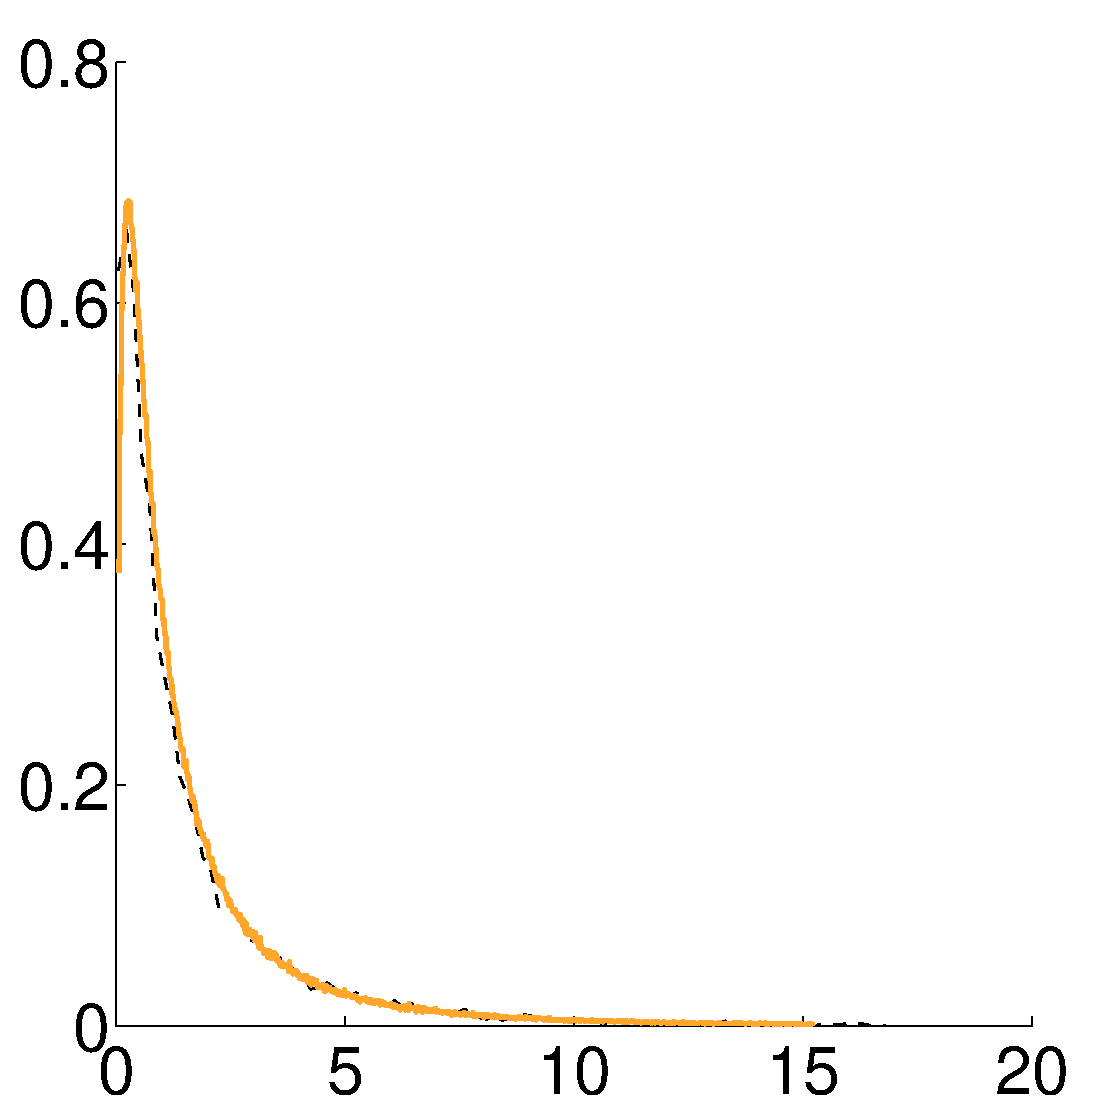
\includegraphics[width=1.5in,height=1.5in]{../images/verify_change_ratio_model_on_RADARSAT2_3d.eps}}

\psset
{
  xunit=\dimexpr\wd\IBox/\column,
  yunit=\dimexpr\ht\IBox/\row,
}

\newcommand{\plotWithLegend}[2]{          
          \begin{pspicture}[showgrid=false](\column,\row)% set showgrid=false for the final
	    \rput[bl](0,0){\includegraphics[width=1.5in,height=1.5in]{#1}}% \usebox\IBoxCRThreeR
	    \rput(5,1.5){\footnotesize{#2}}
	    \rput{90}(1.5,5){\footnotesize{pdf / histogram}}
	    \psline[linecolor=plot](5,8)(6,8)
	    \psline[linestyle=dashed](5,9)(6,9)%another line style: dotted
	    \rput(8,8){\footnotesize{model}}
	    \rput(8,9){\footnotesize{data}}            
          \end{pspicture}
}

\usepackage{cite} %for citations
\renewcommand{\citedash}{--}
\usepackage{url}

 %this is for math typing (eg: cases)
\usepackage{amsmath}
   \usepackage{amsfonts}   % if you want the fonts
   \usepackage{amssymb}    % if you want extra symbols
\usepackage{epsfig} %for figures

\usepackage[center]{caption}%for captions
\usepackage[caption=false,font=footnotesize]{subfig} %for subfigures

%opening
\title{
  Scalar and Representative Observables for Polarimetric SAR Data
}

%\author{Thanh-Hai Le, Ian McLoughlin}
\author{Thanh-Hai~Le,
        Ian~McLoughlin, 
	and Chan-Hua~Vun%
\thanks{Thanh-Hai~Le and Chan-Hua~Vun are with School of Computer Engineering, 
Nanyang Technological University, Singapore. Ian~McLoughlin is with School of Information Science and Technology,
University of Science and Technology of China.
}% <-this % stops a space
%\thanks{The authors wish to thank Dr. Ken-Yoong Lee and Dr. Timo Brestchneider of EADS Innovation-Works Singapore for 
%	providing us the RADAR-SAT2 imagery used in this paper. }% <-this % stops a space
\thanks{Manuscript received ?, 2013; revised ?.}}

\markboth{IEEE Journal on Selected Topic in Applied Earth Observation and Remote Sensing,~Vol.~?, No.~?, ?~2013}%
{ Le \MakeLowercase{\textit{et al.}}:  Scalar and Representative Observables for Polarimetric SAR Data}

\begin{document}

\maketitle

\begin{abstract}
%Problem statement  
This paper proposes a scalar and representative observable for multi-dimensional POLSAR data,
  from which statistically consistent discrimination measures can be derived.
%What actually were done? and As the result, what is learned?
Specifically, the statistical behaviour of the POLSAR covariance matrix determinant is used
  to derive a scalar and generic statistical model for multi-dimensional POLSAR data,
  which is specifically applicable to the two and three dimensional versions of partial and full monostatic polarimetric SAR data.
As the POLSAR covariance matrix determinant generalizes the SAR intensity towards multiple dimensions,
  the proposed model is able to subsume the traditional SAR intensity model under the umbrella of a unified model. 
%What are the larger implications of the findings presented in this paper?
Consequently, the main beneficial implication of the proposed approach is that
  it provides a consistent theory unifying the currently disconnected proposals for SAR and POLSAR discrimination measures
  which simplifies the adaptation of existing SAR data processing techniques for POLSAR data.
%  it enables the adaptation of many existing SAR data processing techniques for POLSAR data,
%  and at the same time, it provides a consistent theory unifying the seemingly disparate discrimination measure proposals for SAR and POLSAR data.
\end{abstract}

\begin{IEEEkeywords}
Polarimetric Synthetic Aperture Radar, Electromagnetic Modeling, Multidimensional Signal Processing  
\end{IEEEkeywords}

\IEEEpeerreviewmaketitle

\section{Introduction}

%What is the situation, the background context of your research? the BIG problem!
During the past decades, exponential growth in computing power has allowed the once computationally-demanding Synthetic Aperture Radar (SAR)
technology to become a feasible and preferred technique for earth observation applications.
SAR technology has since been extended in a few directions, one of which is polarimetric SAR (POLSAR).
POLSAR extends SAR by exploiting the natural polarization property of Electro-Magnetic (EM) waves,
  leading to the availability of multi-channel POLSAR data, compared to traditional one-channel SAR data.
  

%Research Motivation: Why it is important to solve this problem?
%The POLSAR data, however, is multidimensional and stochastic.
Like SAR data, POLSAR data is stochastic.
Moreover, it is multi-dimensional, making it even harder to interpret.
Under this context, it is therefore important to establish a simple and intuitive understanding of the data.
 Statistical models are undoubtedly crucial in understanding its stochastic nature.
While several %multidimensional 
models have been proposed to describe POLSAR data, they
  unfortunately tend to be complex and not very intuitive due to the multidimensional nature of the data.
Practical POLSAR data processing however, makes heavy use of scalar discrimination measures,
  which should be based on statistically consistent models for scalar and representative observables of the multidimensional data.
It is thus important to establish a scalar and representative observable for this multi-dimensional POLSAR data.
  
%Moreover, to provide theoretical foundation for discrimination measures proposal,
%  statistically consistent models should be derived from this scalar observable.

%How do others solve this problem?
%The complex POLSAR data have been statistically modelled as following the complex Wishart distribution,
%  which apparently is multidimensional, complex and thus not very intuitive.
There has been a few scalar observables with accompanying statistical models proposal for POLSAR \cite{Conradsen_2003_TGRS_4, Alberga_2008_IJRS_4129, Joughin_1994_TGRS_562, Lee_1994_TGRS_1017, Touzi_1996_TGRS_519, Lopez-Martinez_2003_TGRS_2232, Erten_2012_Sensors_2766},
  but none of them is able to provide meaningful scalar discrimination measures.
%  but none of them has led to scalar discrimination measures proposal.
As such no observable has been widely accepted as being highly representative of this multi-dimensional data,
  which severely limits their applicability in practical data processing applications.
From an alternative approach, a few POLSAR discrimination measures have been proposed,
  but all are based on the likelihood ratio statistics.
This statistical test should be based on an exact and consistent statistical distribution
  but so far has only shown to be based on an asymptotic distribution.

%Research Objective: Give your precise problem statement  
This article hence presents a scalar and representative observable, and its associated generic statistical model to describe multi-dimensional POLSAR data and provide a consistent foundation for the derivation of POLSAR discrimination measures.
%Now State your approach  
%This study started off with the observation that the determinant of the covariance matrix is widely used in POLSAR discrimination measures.
%However, our survey of existing scalar models for POLSAR indicates that no statistical model for this observable has been published so far.
%Consequently, in this article, the statistical behaviour of the determinant of POLSAR covariance matrix is further investigated.
%Prof Vuns: comment: the article provides the result, not the journey!
POLSAR data have been statistically modelled as following the complex Wishart distribution.
Consequently, the generic statistical model for the covariance matrix determinant is presented as being just a scalar projection of the multidimensional data.
This model is then used to derive several scalar and consistent statistical descriptions suggesting that their associated observables are capable of being used as discrimination measures for POLSAR data.
%
%***IVM: the following sentence doesn't make sense, also, I don't think it's good to talk about 'models of a model'.  Maybe 'model variants' instead?
%%%***IVM***The specific two and three dimensional models of these models, which %also include the derived discrimination measures, are originally designed against both partial and full polarimetric SAR data.

%The specific two and three dimensional models are then validated against both partial and full polarimetric SAR data.
Interestingly the paper also shows that %It is also shown that
  the specific one dimensional versions of the proposed  models 
  match perfectly with the traditional statistical model used for SAR intensity.
This effectively incorporates the common one dimensional SAR theory under the unbrella of the proposed scalar approach for multi dimensional POLSAR.
With this new insight the different discrimination proposals for SAR and POLSAR are reviewed and it is shown that the approach proposed in this paper provides a strong, unifying and consistent foundation relating them all together.
The applicability of these theoretical models will be illustrated by experiments where the specific one, two and three dimensional versions of the proposed generic models are validated against practical data. 
%Furthermore, the approach proposed in this paper
%  not only provides a consistent foundation for the different discrimination measures proposal in POLSAR
%  but also leads to the establishment of a new discriminating measures: the determinant-ratio and the change-ratio.

%What is the novelty of your solution? What are its advantages
%Compared to other published scalar observables with accompanying statistical model,
%  the proposed observable and its models are highly representative of the multidimensional data.
%The representative power of the proposed observable is justified by the following reasons.
%Firstly, the covariance matrix determinant, when collapsed into one-dimensional case, transforms neatly into the representative SAR intensity.
%Secondly, the statistical model for this observable is shown as the generic multi-dimensional extension of the traditional and representative intensity model for the one dimensional SAR data.
%And last but not least, this observable also leads to the determinant-ratio discrimination measure which
%  not only is simpler in concept and computation than the existing POLSAR discrimination measures
%  but also can be considered as the natural multi-dimensional extension of the commonly-used intensity-ratio discrimination measure in SAR.
% Prof Vun Comment: already mentioned above, no need to repeat
%hai thoughts: actually this should be included to justify our title, and our approach. It is however being moved to discussion / conclusion section

%How do you know if the problem is solved? State your research contribution to be achieved
%In summary, the main objective of this article is to propose the determinant of the POLSAR covariance matrix as a scalar observable
%  that is representative of the multi-dimensional data.
%Specifically the following research results are to be achieved:
%  1. The generic scalar and representative statistical model for the determinant of the multi-dimensional POLSAR covariance matrix is to be derived, 
%  2. This generic model is also shown leading to staititically consistent models for newly proposed POLSAR observables, namely the determinant-ratio and the change-ratio.
%  3. The special one-dimensional version of the derived generic model is to be shown perfectly matches with the traditionally used SAR intensity model,
%  4. All specific one, two and three dimensional versions of the derived generic model are to be validated against real-life captured data,
%(Hai NOTE: I kept this to keep my focus while working on this paper.
%  It can be removed before the final submission.)
  
%Article Organization: Show that you deliver on the objectives and hence solve the stated problem
The remainder of this article is organized as follows.
After the next section reviews existing discrimination measures as well as scalar observables models for POLSAR, section \ref{sec:theoretical_model}
  derives the generic statistical model for the determinant of the POLSAR covariance matrix
  and proposes several new discrimination measures for the multi-dimensional data.
After section \ref{sec:sar_special_case_of_polsar} illustrates the match between the specific model of one dimensional and the traditional model for SAR intensity,
  section \ref{sec:link_sar_polsar} links the disparate discrimination measure proposals for the traditional SAR and the more recent POLSAR data.
%Section \ref{sec:polsar_models_validation} then validates the specific one, two and three dimensional versions of the proposed model against real-life captured data.
The applicability of these models against practical data is illustrated in section \ref{sec:polsar_models_validation}.
Section \ref{sec:discussion} presents a high-level discussion of the results presented before
  section \ref{sec:conclusion} finally concludes the paper.

\section{Related Work in Literature}
\label{sec:lit_review}

%This section outlines related publication.
Section \ref{sec:lit_models} reviews various statistical models used for different scalar observables for POLSAR.
  where it is shown that none are able to provide statistically consistent discrimination measures. 
Section \ref{sec:lit_measures} further strengthens those findings by discussing discrimination measures that have been proposed for POLSAR,
  and demonstrates that almost all of them are based on the likelihood statistical test for complex Wishart distribution.
While an exact statistical distribution is expected to be necessary for a test,
  only an asymptotic distribution is used in the underlying approach \cite{Conradsen_2003_TGRS_4}.
  
\subsection{Scalar Observables for POLSAR Data and their Statistical Models}
\label{sec:lit_models}

Different target decomposition theorems have identified many possible scalar observables for complex POLSAR data.
In \cite{Alberga_2008_IJRS_4129}, the performance of different scalar POLSAR observables is evaluated for classification purposes.
While many scalar observables for POLSAR were presented, their corresponding statistical models and classifiers were not available.
Furthermore, at its conclusion, the paper indicated that it is impossible to identify a single best representation.
Although, to be fair, the observables were identified for describing a decomposed portion of the complex POLSAR data,
  rather than providing a unified representation of the POLSAR data.

Using a different approach, given that the joint distribution for POLSAR is known to be the multi-variate complex Wishart distribution,
  it is possible to derive the scalar statistical models for some univariate POLSAR observables.
%This becomes an alternative approach used in the study of POLSAR data.
However, such derivations are not trivial tasks, and so far, only a handful of such statistical models have been proposed, including the following:
  \begin{enumerate}
  \item cross-pol ratio $r_{HV/HH} = |S_{HV}|^2/|S_{HH}|^2$ \cite{Joughin_1994_TGRS_562},
  \item co-pol ratio $r_{VV/HH} = |S_{VV}|^2/|S_{HH}|^2$ \cite{Joughin_1994_TGRS_562},
  \item co-pol phase difference $\phi_{VV/HH} = arg(S_{VV}S_{HH}^*) $ \cite{Joughin_1994_TGRS_562} \cite{Lee_1994_TGRS_1017},
  \item magnitude $g=|avg(S_{pq}S_{rs}^*)|$ \cite{Lee_1994_TGRS_1017},
  \item normalized magnitude $\xi = \frac{|avg(S_{pq}S_{rs}^*)|}{\sqrt{avg(|S_{pq}|^2) avg(|S_{rs}|^2)}}$ \cite{Lee_1994_TGRS_1017},
  \item intensity ratio $w = avg(|S_{pq}|^2)/avg(|S_{rs}|^2)$ \cite{Lee_1994_TGRS_1017},
  \item and the Stokes parameters $S_i,0 \leq i \leq 3$ \cite{Touzi_1996_TGRS_519}. 
  \end{enumerate}
More recently, statistical models for
  each element of the POLSAR covariance matrix, i.e. $S_{pq}S_{rs}^*$, \cite{Lopez-Martinez_2003_TGRS_2232}
  as well as for the largest eigen-value of the covariance matrix $\lambda_1$ \cite{Erten_2012_Sensors_2766} have been proposed.

While these models undoubtedly help to further our understandings of the POLSAR data,
  none of the underlying observables have been shown to meet the dual criteria of
  1) resulting in statistically consistent discrimination measures and thus 
  2) being representative of the complex POLSAR data.

\subsection{POLSAR Discrimination Measures}
\label{sec:lit_measures}

The commonly used measure of distance for matrices are either the Euclidean or Manhattan distances, defined respectively as:
\begin{align}
  d(C_x,C_y) &= \sum_{i,j} |\mathbb{R} (C_x - C_y)_{i,j}| + \sum_{i,j} |\mathbb{I} (C_x - C_y)_{i,j}| \\
  d(C_x,C_y) &= \sqrt{\sum_{i,j} |C_x - C_y|_{i,j}^2 }
\end{align}
where $C_{i,j}$ denotes the $(i,j)$ elements of the POLSAR covariance matrix C,
 $||$ denotes absolute values
and $\mathbb{R},\mathbb{I}$ denote the real and imaginary parts respectively.
However, in the context of POLSAR, % covariance matrix
  these dissimilarity measures are not widely used 
  mainly due to the multiplicative nature of the noisy data.

In the field of POLSAR, the Wishart distance is probably the most widely used, as part of the well-known Wishart classifier \cite{Lee_1999_TGRS}.
It is defined \cite{Lee_1994_IJRS_2299} as:
\begin{equation}
  d(C_x,C_y) = \ln|C_y| + tr(C_xC_y^{-1})
\end{equation},
where $tr(C)$ denotes the trace of the matrix C. 
As a measure of distance, its main disadvantage is that $d(C_y,C_y) = \ln|C_y| \neq 0$.

Recent works have suggested alternative dissimilarity measures including the symmetric and asymmetric refined Wishart distance \cite{Anfinsen_2007_ESA_POLINSAR},
\begin{align}
  d(C_x,C_y) &= \frac{1}{2} tr(C_x^{-1}C_y + C_y^{-1}C_x) - d \\
    d(C_x,C_y) &= \ln|C_x| - \ln|C_y| + tr(C_xC_y^{-1}) - d
\end{align}
the Bartlett distance \cite{Kersten_2005_TGRS_519},
  \begin{align}
  d(C_x,C_y) &= 2 \ln |C_{x+y}| - \ln |C_x| - \ln |C_y| - 2d\ln2
  \end{align}
the Bhattacharyya distance \cite{Lee_2011_IGARSS_3740},
\begin{equation}
  r(C_x,C_y) = \frac{|C_x|^{1/2} |C_y|^{1/2}}{|(C_x+C_y)/2|}
\end{equation}
and the Wishart Statistical test distance \cite{Cao_2007_TGRS_3454}
\begin{equation}
  d(C_x,C_y) = (L_x + L_y) \ln|C| - L_x \ln|C_x| - L_y\ln|C_y|
\end{equation}

Closer examination of these dissimilarity measures reveals that most of them are related in some ways. %to each other.
The Bhattacharyya distance is easily shown to be related to the Barlett distance.
At the same time the Barlett distance can be considered a special case of the Wishart Statistical Test distance,
  when the two data sets have the same number of looks, i.e. $L_x=L_y$.
The close relation among the measures is further supported by the fact that
  all of their publications refered the same statistical model developed in \cite{Conradsen_2003_TGRS_4} as the foundation.
In \cite{Conradsen_2003_TGRS_4}, to determine if the two scaled multi-look POLSAR covariance matrixes $Z_x$ and $Z_y$,
  which have $L_x$ and $L_y$ as the corresponding number of looks,
  come from the same underlying stochastic process,
the likelihood ratio statistics for POLSAR covariance matrix is considered:  
\begin{equation*}
  Q = \frac{(L_x+L_y)^{d \cdot (L_x+L_y)}}{L_x^{d \cdot L_x} L_y^{d \cdot L_y}} \frac{|Z_x|^{L_x} |Z_y|^{L_y} }{|Z_x+Z_y|^{(L_x+L_y)}}
\end{equation*}

Taking the log-transformation of the above equation, and denoting $C_{vx} = Z_x / L_x$, $C_{vy} = Z_y / L_y$ and $C_{vxy} = (Z_x + Z_y)/(L_x + L_y)$ then:
{\small
\begin{align}
  Q &= \frac{|C_{vx}|^{L_x} \cdot |C_{vy}|^{L_y} }{|C_{vxy}|^{L_x + L_y}} \label{eqn:ori_likelyhood_stats} \\
  \ln Q &= L_x \ln |C_{vx}| + L_y \ln |C_{vy}| - (L_x + L_y) \ln |C_{vxy}| \label{eqn:log_likelyhood_stats}
\end{align}
}

To detect changes, a test statistic is developed for this discrimination measure.
This means a distribution is to be derived for the dissimilarity measure.
However, in the original work \cite{Conradsen_2003_TGRS_4}, only an asymptotic distribution was used.
This paper proposes a statistical model for the determinant of the POLSAR covariance matrix $|C_v|$
  which is capable of providing an exact distribution for the test.

\section{The Generic Scalar Statistical Model for POLSAR}  
\label{sec:theoretical_model}

%In this section, the generic scalar statistical model for POLSAR is presented.
In this section, after the basic foundations of POLSAR statistical analysis are introduced,
  the generic scalar statistical model for the multi-dimensional POLSAR will be presented.
%  this section presents the theoretical model for multi-dimensional POLSAR data. 

In this paper, the POLSAR scattering vector is denoted as $s$.
For partial polarimetric SAR (single polarization in transmit and dual polarization in receipt),
  the vector is two-dimensional ($d=2$) and is normally written as: 
\begin{equation}
s_{part}=\begin{bmatrix}
S_h\\ 
S_v
\end{bmatrix}
\end{equation}
For full and monostatic POLSAR data,
  the vector is three-dimensional ($d=3$) and is presented as:
\begin{equation}
s_{full}=\begin{bmatrix}
S_{hh}\\
\sqrt{2}S_{hv}\\
S_{vv}
\end{bmatrix}
\end{equation}

Let $\Sigma=E [ss^{*T}]$ denote the population expected value of the POLSAR covariance matrix,
  where $s^{*T}$ is the complex conjugate transpose of $s$. 
Assuming %all the elements in $s$ are independent and
  $s$ is jointly circular complex Gaussian with the expected covariance matrix $\Sigma$,
  then the probability density function (PDF) of $s$ can be written as:
\begin{equation}
  pdf(s;\Sigma)=\frac{1}{\pi^d|\Sigma|} e^{-s^{*T}\Sigma^{-1}s}
\end{equation}
where $||$ denotes the matrix determinant.

The sample POLSAR covariance matrix is formed as the mean of Hermitian outer product of independent single-look scattering vectors,
\begin{equation}
  C_v = \langle ss^{*T} \rangle = \frac{1}{L} \sum^L_{i=1}s_is_i^{*T}
\end{equation}
where $L$ is the number of looks
  and $s_i$ denotes the single-look scattering vector,
  which equals $s_{part}$ for the case of partial POLSAR or
  $s_{full}$ for the case of full polarimetry.

Complex Wishart distribution statistics are normally used for the scaled covariance matrix
$Z=LC_v$, whose PDF is given as:
\begin{equation}
  pdf(Z;d,\Sigma,L)=\frac{|Z|^{L-d}}{|\Sigma^L|\Gamma_d(L)}e^{-tr(\Sigma^{-1}Z)}
\end{equation}
with $\Gamma_d(L) = \pi^{d(d-1)/2} \prod^{d-1}_{i=0}\Gamma(L-i)$
and $d$ is the dimensional number of the POLSAR covariance matrix.

The approach taken in this paper differs by applying the homoskedastic log transformation  on a less-than-well-known result for the determinant of the covariance matrix.
Goodman \cite{Goodman_1963_AMS_178} proved
that the ratio between the observable and expected values of the sample covariance matrix determinants
  behaves like a product of $d$ chi-squared random variables with different degrees of freedom: 
\begin{equation}
\chi^d_L = (2L)^d \frac{|C_v|}{|\Sigma_v|} \sim \prod_{i=0}^{d-1} \chi (2L-2i)
\label{eqn:prod_chi_squared_rv}  
\end{equation}

%We will now use 
This result is used here to develop the generic scalar statistical model for POLSAR. %log-transformed measures of distance.
From Eqn. \ref{eqn:prod_chi_squared_rv} %and \ref{eqn:sum_log_chi_squared_rv}
we have: %can deduce the following relationships:
\begin{eqnarray}
  |C_v| &\sim& |\Sigma_v| \cdot \frac{1}{(2L)^d} \cdot \prod_{i=0}^{d-1} \chi (2L-2i) \label{eqn:determinant_distribution} %\\
%  \ln|C_v| &\sim& \ln|\Sigma_v| - d \cdot \ln(2L) + \sum^{d-1}_{i=0} \Lambda(2L-2i)
%\label{eqn:log_determinant_distribution}  
\end{eqnarray}

In a given homogeneous POLSAR area, the parameters $\Sigma_v$, $d$ and $L$ can be considered constant.
Thus Eqn. \ref{eqn:determinant_distribution} indicates that 
  in the original POLSAR domain, a multiplicative speckle noise pattern is present.

Moreover, since the average and variance of these chi-squared distributions %and log-chi-squared distribution
  are known to be constant, i.e. $avg \left[ \chi(2L) \right] = 2L$ and $var \left[ \chi(2L) \right] = 4L$,
  the product and summation of these random variables also have fixed summary statistics.
Specifically:
{\footnotesize
\begin{align*}
  avg \left[ \prod^{d-1}_{i=0} \chi(2L-2i) \right] &= 2^d \cdot \prod^{d-1}_{i=0} (L-i), \\
  var \left[ \prod^{d-1}_{i=0} \chi(2L-2i) \right] &= \prod^{d-1}_{i=0} 4(L-i)(L-i+1) - \prod^{d-1}_{i=0} 4(L-i)^2, %\\
%  avg \left[ \sum^{d-1}_{i=0} \Lambda(2L-2i) \right] &= d \cdot \ln{2} + \sum^{d-1}_{i=0} \psi^0(L-i), \\
%  var \left[ \sum^{d-1}_{i=0} \Lambda(2L-2i) \right] &= \sum^{d-1}_{i=0} \psi^1(L-i)
\end{align*}
}

Combining these results with Eqn. \ref{eqn:determinant_distribution} %and \ref{eqn:log_determinant_distribution}
  , we have:
{\footnotesize
\begin{align}
  avg \left[ |C_v| \right]  &= \frac{|\Sigma_v|}{L^d} \prod^{d-1}_{i=0} (L-i)\\
  var \left[ |C_v| \right]  &=   \frac{|\Sigma_v|^2 \left[ \prod^{d-1}_{i=0} (L-i)(L-i+1) - \prod^{d-1}_{i=0} (L-i)^2 \right] }{L^{2d}} \label{eqn:var_det_is_heteroskedastic}%\\
%  avg \left[ \ln |C_v| \right] &= \ln |\Sigma_v| - d \cdot \ln{L}  + \sum^{d-1}_{i=0} \psi^0(L-i) \label{eqn:avg_log_det} \\
%  var \left[ \ln |C_v| \right] &=  \sum^{d-1}_{i=0} \psi^1(L-i) \label{eqn:var_log_det_is_homoskedastic}
\end{align}
}

For a real world captured image, while the parameters $d$ and $L$ do not change for the whole image,
  the underlying $\Sigma_v$ is expected to differ from one region to the next.
Thus over a heterogeneous scene, the stochastic process for $|C_v|$ and $\ln |C_v|$ vary depending on the underlying signal $\Sigma_v$. 
In such context, Eqn. \ref{eqn:var_det_is_heteroskedastic} implies that the variance of $|C_v|$ also differs depending on the underlying signal $\Sigma_v$ (i.e. it is   heteroskedastic).

Similar to the way intensity-ratio is proposed as the discrimination measure for the multiplicative and heteroskedastic SAR intensity \cite{Rignot_1993_TGRS_896},
in this paper, the determinant-ratio and the change-ratio are also proposed as a discrimination measure for the POLSAR data.
  which is shown above to also suffer from the multiplicative and heteroskedastic phenomena.
%Similar to the way dispersion and contrast is defined for one-dimensional SAR \cite{Le_2010_ACRS},
%  this section introduces the consistent sense of distance for POLSAR.

%Assuming, on the one hand,
For cases where the true value of the underlying signal $\Sigma_v$ is known \textit{a priori},
then the determinant-ratio of the signal random variable ($\mathbb{R}_{\Sigma}$) %and log-distance ($\mathbb{L}$)
%  are observable according to the following definitions:
  is defined as:
%Eqns. \ref{eqn:prod_chi_squared_rv} and \ref{eqn:sum_log_chi_squared_rv} lead straight to the definition of the following random variables, which is the :
\begin{eqnarray}
  \mathbb{R}_{\Sigma} &=& \frac{|C_v|}{|\Sigma_v|} \label{eqn:determinant_ratio_observables}%\\
%  \mathbb{L} &=& \ln|C_v| - \ln|\Sigma_v| \label{eqn:log_distance_observables} 
\end{eqnarray}
%On the other hand, under a looser assumption %From another perspective
For cases where the POLSAR data is known to have come from a homogeneous area, but the true value of the underlying signal $\Sigma_v$ is \textit{unknown},
 then a random variable called the change-ratio ($\mathbb{R}_{C}$)  is defined as:
\begin{eqnarray}
  \mathbb{R}_{C} &=& \frac{|C_1|}{|C_2|} \label{eqn:determinant_ratio_samples_observables}%\\
%  \mathbb{L} &=& \ln|C_v| - \ln|\Sigma_v| \label{eqn:log_distance_observables} 
\end{eqnarray}
where $C_1$ and $C_2$ are samples of the covariance matrix determinant in an assumed homogeneous area. 

%  the dispersion ($\mathbb{D}$) and contrast ($\mathbb{C}$) random variables are the observables defined as:
%\begin{eqnarray}
%  \mathbb{D} &=& \ln{|C_v|} - avg(\ln{|C_v|}) \label{eqn:dispersion_observable}\\
%  \mathbb{C} &=& \ln(|C_{v1}|) - \ln(|C_{v2}|) \label{eqn:contrast_observable}
%\end{eqnarray}

Using the results from Eqn. \ref{eqn:determinant_distribution}, %\ref{eqn:log_determinant_distribution} and \ref{eqn:avg_log_det}
  we have
\begin{eqnarray}
\mathbb{R}_{\Sigma} &\sim& \frac{1}{(2L)^d} \cdot \prod_{i=0}^{d-1} \chi (2L-2i) \label{eqn:determinant_ratio_distribution} \\
\mathbb{R}_{C} &\sim& \prod_{i=0}^{d-1} \frac{\chi(2L-2i)}{\chi(2L-2i)} \label{eqn:change_ratio_distribution}
%\mathbb{L} &\sim&  \sum^{d-1}_{i=0} \Lambda(2L-2i) - d \cdot \ln(2L)
%\label{eqn:log_determinant_distance_distribution} \\ 
% \mathbb{D} &\sim& \sum^{d-1}_{i=0} \Lambda(2L-2i) - d \cdot \ln{2} + k
%\label{eqn:dispersion_distribution} \\ 
% \mathbb{C} &\sim& \sum^{d-1}_{i=0} \Delta(2L-2i)
%\label{eqn:contrast_distribution}  
\end{eqnarray}
%with $\Delta(2L) \sim \Lambda(2L) - \Lambda(2L)$
%and $k=\sum^{d-1}_{i=0} \psi^0(L-i)$

%Thus the characteristic functions for the summative random variables is derived in Appendix \ref{sec:appendix_b} as:
%\begin{align}
%  CF_{\Lambda^d_L}(t) &= \frac{2^{idt}}{\Gamma(L)^d} \prod^{d-1}_{j=0} \Gamma(L-j+it) \\
%  CF_{\mathbb{L}}(t) &= \frac{1}{L^{idt} \Gamma(L)^d} \prod^{d-1}_{j=0} \Gamma(L-j+it) \\
%  CF_{\mathbb{D}}(t) &= \frac{e^{ikt}}{\Gamma(L)^d} \prod^{d-1}_{j=0} \Gamma(L-j+it) \\
%  CF_{\Delta(2L)} &= \frac{\Gamma(2L) B(L-it,L+it)}{\Gamma(L)^2} \\
%  CF_{\mathbb{C}}(t) &=  \prod^{d-1}_{j=0} \frac{\Gamma(2L-2j) B(L-j-it,L-j+it)}{\Gamma(L-j)^2}
%\end{align}

Since each elementary component follows fixed distributions (i.e. $\chi^2(2L)$),
  it is natural that this variable also follows fixed distributions.
Moreover, it is independent of the underlying signal $\Sigma_v$,
  indicating its statistically consistent properties and hence its applicability as a POLSAR discrimination measure.
This claim is extrapolated from the widely-used intensity-ratio as a SAR discrimination measure
  and will be further discussed in the next sections.
%is further strengthened in the next section which shows that the generic models for POLSAR presented in this paper also include the commonly-used models for SAR as its special 1-dimensional case. 
%This result shows how
%In short, these random variables are shown to follow consistent and fixed distributions,
%  regardless of the underlying signal $\Sigma_v$.

\section{SAR as a one-dimensional case of POLSAR}
\label{sec:sar_special_case_of_polsar}

%The previous sections have introduced and validated the theoretical models for 3-dimensional ($d=3$) full polarimetric and 2-dimensional ($d=2$) partial polarimetry, cases.
This section shows that the proposed generic model is equally  applicable to the 1-dimensional ($d=1$) case,
  which is physically equivalent to  collapsing the multi-dimensional POLSAR dataset  into conventional single dimensional SAR data.
Mathematically, the sample covariance matrix $C_v$ is reduced to the sample variance while the determinant $|C_v|$ is equivalent to  the scalar variance value.
As variance is equal to intensity $I$ for SAR data, our result is consistent with previous results for SAR intensity data.
Thus the proposed generic model for POLSAR, collapsed into one dimension will be shown to incorporate the traditional SAR intensity as a natural case of the unified model.
%  as well as reminding us that SAR is a special case of POLSAR.
  
The results for our models can be summarized using the following equations:
\begin{align*}
  |C_v| &\sim |\Sigma_v| \cdot \frac{1}{(2L)^d} \cdot \prod_{i=0}^{d-1} \chi (2L-2i) \\ %\label{eqn:determinant_distribution} %\\
  \mathbb{R}_{\Sigma} = \frac{|C_v|}{|\Sigma_v|} &\sim \frac{1}{(2L)^d} \prod^{d-1}_{i=0} \chi(2L-2i) \\ %\label{eqn:polsar_ratio_det_cov_dist} \\
\mathbb{R}_{C} = \frac{C_1}{C_2} &\sim \prod_{i=0}^{d-1} \frac{\chi(2L-2i)}{\chi(2L-2i)}
%  \mathbb{L} &= \ln{|C_v|} - \ln{|\Sigma_v|} \sim \sum^{d-1}_{i=0} \Lambda(2L-2i) - d \cdot \ln{2L} \\ %\label{eqn:polsar_dispersion_log_det_cov_dist} \\
%  \mathbb{D} &= \ln{|C_v|} - avg(\ln{|C_v|}) \sim \sum^{d-1}_{i=0} \Lambda(2L-2i) - d \ln{2} + k\\
%  \mathbb{C} &= \ln{|C_{1v}|} - \ln{|C_{2v}|} \sim \sum^{d-1}_{i=0} \Delta(2L-2i) \\
%  \mathbb{A} &= avg(\mathbb{L}) = \sum^{d-1}_{i=0} \psi^0(L-i) - d \cdot \ln{L} \\ %\label{eqn:polsar_dispersion_averages} \\
%  \mathbb{V} &= var(\mathbb{L}) = \sum^{d-1}_{i=0} \psi^1(L-i) \\ %\label{eqn:polsar_dispersion_variance} \\
%  \mathbb{E} &= mse(\mathbb{L}) =\left[ \sum^{d-1}_{i=0} \psi^0(L-i) - d \cdot \ln{L} \right]^2 +  \sum^{d-1}_{i=0} \psi^1(L-i) \label{eqn:polsar_dispersion_mse} 
\end{align*}

Upon setting $d=1$ into the above equations,
  the equations become:
\begin{align*}
  |C_v| &\sim  \frac{|\Sigma_v|}{(2L)} \cdot \chi (2L) \\ %\label{eqn:determinant_distribution} %\\
  \mathbb{R}_{\Sigma} = \frac{|C_v|}{|\Sigma_v|} &\sim \frac{1}{(2L)} \cdot \chi(2L) \\ %\label{eqn:polsar_ratio_det_cov_dist} \\
\mathbb{R}_{C} = \frac{C_1}{C_2} &\sim \prod_{i=0}^{d-1} \frac{\chi(2L-2i)}{\chi(2L-2i)}
\end{align*}

Since the PDF of chi-squared distribution can be written as:
\begin{align*}
\chi(2L) \sim pdf \left[ \frac{\chi^{L-1}e^{-\chi/2}}{2^L\Gamma(L)} \right]
\end{align*}
Applying variable change theorem into the above equations results in:
\begin{align*}
  |C_v| &\sim  pdf \left[ \frac{L^L x^{L-1} e^{-Lx/|\Sigma_v|}}{\Gamma(L) |\Sigma_v|^L} \right] \\ %\label{eqn:determinant_distribution} %\\
  \mathbb{R}_{\Sigma} = \frac{|C_v|}{|\Sigma_v|} &\sim pdf \left[ \frac{ L^{L} x^{L-1} e^{-Lx}}{ \Gamma(L)} \right] \\ %\label{eqn:polsar_ratio_det_cov_dist} \\
  \mathbb{R}_{C} = \frac{C_1}{C_2} &\sim pdf \left[ \frac{\Gamma(2L-1) x^{L-1}}{\Gamma^2(L-1) (1+x)^{2L}} \right]
\end{align*}
These equations match exactly with the following traditional model for multi-look SAR intensity:
  \begin{eqnarray}
I &\sim& pdf \left[ \frac{L^L x^{L-1} e^{-Lx/\bar{I}}}{\Gamma(L) \bar{I}^L} \right] \\
\mathbb{R}_{\bar{I}} = \frac{I}{\bar{I}} &\sim& pdf \left[ \frac{ L^{L} x^{L-1} e^{-Lx}}{ \Gamma(L)} \label{eqn:multi_look_SAR_ratio_dist} \right] \\
  \mathbb{R}_{I} = \frac{I_1}{I_2} &\sim& pdf \left[ \frac{\Gamma(2L-1) x^{L-1}}{\Gamma^2(L-1) (1+x)^{2L}} \right]
  \end{eqnarray}
considering that $|C_v| \mapsto I$ and $|\Sigma_v| \mapsto \bar{I}$ as multi-dimensional POLSAR collapses into single-dimensional SAR.

\section{Unifying the different discrimination measures proposals for both SAR and POLSAR}
\label{sec:link_sar_polsar}

Statistical models have always been the foundation for deriving discrimination measures.
This is true for both fields of SAR and POLSAR.
For SAR, where the field is more or less settled on the issue,
  the statistical model for SAR intensity has been used to derive the most widely used intensity-ratio discrimination measure \cite{Rignot_1993_TGRS_896}.
For POLSAR, where the research field is much less mature,
  the same case should apply, 
  except that so far only asymptotic distributions have been derived for the most common foundation, i.e. the likelihood test statistics \cite{Conradsen_2003_TGRS_4}.

With the insight gained from section \ref{sec:sar_special_case_of_polsar}, this section presents a few results.
%  it should be clear that the proposed model can also be used to derive discrimination measures for POLSAR.
First, similar to the way that the statistical model for SAR intensity has been used to provide the foundation for SAR discrimination measures, e.g. intensity-ratio \cite{Rignot_1993_TGRS_896},
  the statistical model proposed for POLSAR covariance matrix determinant is to be reviewed as providing the foundation for POLSAR discrimination measures, i.e. the likelihood test statistics.
And second, new discrimination measures for POLSAR may be derived by learning from the existing SAR discrimination measures.

As for the first matter, in view of the models given in Eqn \ref{eqn:determinant_distribution},
  the likelihood test statistics presented in \cite{Conradsen_2003_TGRS_4} and rewritten in Eqns \ref{eqn:ori_likelyhood_stats} \& \ref{eqn:log_likelyhood_stats}
can be expressed as:
\begin{align*}
  \ln{Q} &\sim  k + L_x \Lambda^d_{L_x} + L_y \Lambda^d_{L_y} - (L_x + L_y) \Lambda^d_{(L_x + L_y)} \\
  Q &\sim e^k \frac{(\chi^d_{L_x})^{L_x} \cdot (\chi^d_{L_y})^{L_y}}{(\chi^d_{L_x + L_y})^{L_x + L_y}}   
\end{align*}
where $k = d \left[ (L_x + L_y) \ln(L_x + L_y) - L_x \ln{L_x} - L_y \ln{L_y} \right]$.
This, in essence, derives an exact statistical distribution for the likelihood test statistics,
  as opposed to the asymptotic distribution derived in \cite{{Conradsen_2003_TGRS_4}}.

As a by-product of this exact derivation,
  several discrimination measures for the common case of $L_x=L_y$ are further proposed.
They are the determinant-ratio and the change-ratio presented in Section \ref{sec:theoretical_model}.
Compared to existing discrimination measures for POLSAR reviewed in Section \ref{sec:lit_review}, 
  the proposed dissimilarity measures are simpler in both concept and computation.
They, at the same time, are multi-dimensional extensions of the intensity-ratio discrimination measure widely used in SAR.

In short, with the newly gained insight,
  the approach proposed in this paper provides a new bridge between the two fields of SAR and POLSAR.
This invites the adaptation of many established SAR data processing techniques towards POLSAR data,
  where this Section has just described a few examples.
However, before further discussion ensues, 
  it is necessary to validate the presented theoretical model with real-life practical data.

\section{Validating the proposed models against real-life data}
\label{sec:polsar_models_validation}

This section aims to verify the theoretical models given in Eqns. \ref{eqn:determinant_distribution}, \ref{eqn:determinant_ratio_distribution} and \ref{eqn:change_ratio_distribution} against practical data.
All of these models require the estimation of two parameters from the captured data.
These are (i) the dimensional number $d$ and (ii) the look number $L$.
The dimensional number $d$ is related to the type of (POL)SAR data captured,
  with $d=1,2,3$ corresponding to the cases of SAR, partial and full polarimetric SAR data, respectively.
The look-number $L$ can be taken either as nominally stated by the data provider,
  or it can be estimated using the technique proposed by \cite{Anfinsen_2009_TGRS_3795}.

To show the robustness of the proposed models, 
  their validations are also put to test on different types of POLSAR sensors.
Specifically in this paper, the air-borne four-look ($L=4$) AIRSAR image of Flevoland and
  a fine-quad single-look complex RADARSAT2 image ($L=1$) are used.
Since the determinant of the covariance matrix is only significant on multi-look data,
  nine-look processing is first applied on the single-look RADARSAT2 data ($L=9$).

\subsection{The Traditional case of SAR ($d=1$)}

Since it has been shown in Section \ref{sec:sar_special_case_of_polsar} that the model for the case of $d=1$ matches exactly with the traditional model for SAR intensity,
  the validation of the proposed $d=1$ model is quite straightforward. %only a simple validation is presented for this case.  
Fig. \ref{fig:verify_POLSAR_model_1D} presents the results of a test performed for the stated purpose.
In the test, the intensity of single-channel SAR data (HH) for sample homogeneous areas in both datasets is extracted.
The histograms for both the intensity and intensity ratio %the log-distance and contrast
  are then plotted against the theoretical PDF given above.
%Also presented are the plots of the same test applied on a homogeneous patch inside the nine-look processed RADARSAT2 image.
The plots are obtained having set ENL to an estimated value obtained using the technique presented in \cite{Anfinsen_2009_TGRS_3795}.
In all cases, the good visual match between the actual data and model distribution tends to validate the proposed model. %providing us a simple validation of the result.

\begin{figure}[h]
\centering
\begin{tabular}{c}
	\subfloat[AIRSAR (HH) determinant]{
          \plotWithLegend{../images/verify_determinant_model_on_AIRSAR_1d.eps}{determinant}
%		 \epsfxsize=1.5in
%		 \epsfysize=1.5in
%		 \epsffile{../images/verify_determinant_model_on_AIRSAR_1d.eps} 	
		 \label{AIRSAR_1D_determinant}
	} 
	\hfill	
	\subfloat[RADARSAT2 (HH) determinant]{
          \plotWithLegend{../images/verify_determinant_model_on_RADARSAT2_1d.eps}{determinant}
%		 \epsfxsize=1.5in
%		 \epsfysize=1.5in
%		 \epsffile{../images/verify_determinant_model_on_RADARSAT2_1d.eps} 	
		 \label{RADARSAT2_1D_determinant}
	} \\
	\subfloat[AIRSAR (HH) determinant ratio]{
          \plotWithLegend{../images/verify_det_ratio_model_on_AIRSAR_1d.eps}{determinant-ratio}
%		 \epsfxsize=1.5in
%		 \epsfysize=1.5in
%		 \epsffile{../images/verify_det_ratio_model_on_AIRSAR_1d.eps} 	
		 \label{AIRSAR_1D_det_ratio}
	} 
	\hfill	
	\subfloat[RADARSAT2 (HH) determinant ratio]{
          \plotWithLegend{../images/verify_det_ratio_model_on_RADARSAT2_1d.eps}{determinant-ratio}
%		 \epsfxsize=1.5in
%		 \epsfysize=1.5in
%		 \epsffile{../images/verify_det_ratio_model_on_RADARSAT2_1d.eps} 	
		 \label{RADARSAT2_1D_det_ratio}
	} \\
	\subfloat[AIRSAR (HH) change ratio]{
          \plotWithLegend{../images/verify_change_ratio_model_on_AIRSAR_1d.eps}{change-ratio}
%		 \epsfxsize=1.5in
%		 \epsfysize=1.5in
%		 \epsffile{../images/verify_change_ratio_model_on_AIRSAR_1d.eps} 	
		 \label{AIRSAR_1D_det_ratio}
	} 
	\hfill	
	\subfloat[RADARSAT2 (HH) change ratio]{

\plotWithLegend{../images/verify_change_ratio_model_on_RADARSAT2_1d.eps}{change-ratio}
%		 \epsfxsize=1.5in
%		 \epsfysize=1.5in
%		 \epsffile{../images/verify_change_ratio_model_on_RADARSAT2_1d.eps} 	
		 \label{RADARSAT2_1D_det_ratio}
	}
\end{tabular}
\caption{The specific d=1 models are validated for both RADARSAT2 and AIRSAR dataset homogeneous patches}
\label{fig:verify_POLSAR_model_1D}
\end{figure}

\subsection{The Multi-dimensional case of POLSAR ($d=2,3$)}

The remainder of this section now focuses on validating the models for both partial ($d=2$) and full ($d=3$) POLSAR.
Similar tests %like the one described for SAR data 
  are carried out
  for both types of polarimetric SAR
  on both AIRSAR and RADARSAT2 datasets.
The look-number is estimated for each type of data and for each image using the technique described in \cite{Anfinsen_2009_TGRS_3795}. %and is also noted in the plots.
The practical and predicted distributions are again plotted to determine whether their visual match is close in each case. Fig. \ref{fig:verify_det_ratio_model_2D} shows the $d=2$ plots for determinant, determinant ratio and change ratio for both datasets. It is very clear that the model histogram matches the data well, in fact appearing similar to a smoothed data response. Evidently the match is good for $d=2$.

Similarly, Fig. \ref{fig:verify_det_ratio_model_3D} explores the $d=3$ case for the same data, same model parameters. Again, although the histogram is much tighter, the match is visually obvious in all cases.
\begin{figure}[h]
\centering
\begin{tabular}{c}
	\subfloat[AIRSAR (HH-HV) determinant]{
          \plotWithLegend{../images/verify_determinant_model_on_AIRSAR_2d.eps}{determinant}
%		 \epsfxsize=1.5in
%		 \epsfysize=1.5in
%		 \epsffile{../images/verify_determinant_model_on_AIRSAR_2d.eps} 	
		 \label{AIRSAR_2D_determinant}
	} 
	\hfill	
	\subfloat[RADARSAT2 (HH-HV) determinant]{
          \plotWithLegend{../images/verify_determinant_model_on_RADARSAT2_2d.eps}{determinant}
%		 \epsfxsize=1.5in
%		 \epsfysize=1.5in
%		 \epsffile{../images/verify_determinant_model_on_RADARSAT2_2d.eps} 	
		 \label{RADARSAT2_2D_determinant}
	} \\
	\subfloat[AIRSAR (HH-HV) determinant ratio]{
          \plotWithLegend{../images/verify_det_ratio_model_on_AIRSAR_2d.eps}{determinant-ratio}
%		 \epsfxsize=1.5in
%		 \epsfysize=1.5in
%		 \epsffile{../images/verify_det_ratio_model_on_AIRSAR_2d.eps} 	
		 \label{AIRSAR_2D_det_ratio}
	} 
	\hfill	
	\subfloat[RADARSAT2 (HH-HV) determinant ratio]{
          \plotWithLegend{../images/verify_det_ratio_model_on_RADARSAT2_2d.eps}{determinant-ratio}
%		 \epsfxsize=1.5in
%		 \epsfysize=1.5in
%		 \epsffile{../images/verify_det_ratio_model_on_RADARSAT2_2d.eps} 	
		 \label{RADARSAT2_2D_det_ratio}
	} \\
	\subfloat[AIRSAR (HH-HV) change ratio]{
          \plotWithLegend{../images/verify_change_ratio_model_on_AIRSAR_2d.eps}{change-ratio}
%		 \epsfxsize=1.5in
%		 \epsfysize=1.5in
%		 \epsffile{../images/verify_change_ratio_model_on_AIRSAR_2d.eps} 	
		 \label{AIRSAR_2D_det_ratio}
	} 
	\hfill	
	\subfloat[RADARSAT2 (HH-HV) change ratio]{
          \plotWithLegend{../images/verify_change_ratio_model_on_RADARSAT2_2d.eps}{change-ratio}
%\newsavebox\IBoxCRTwoR
%\savebox\IBoxCRTwoR{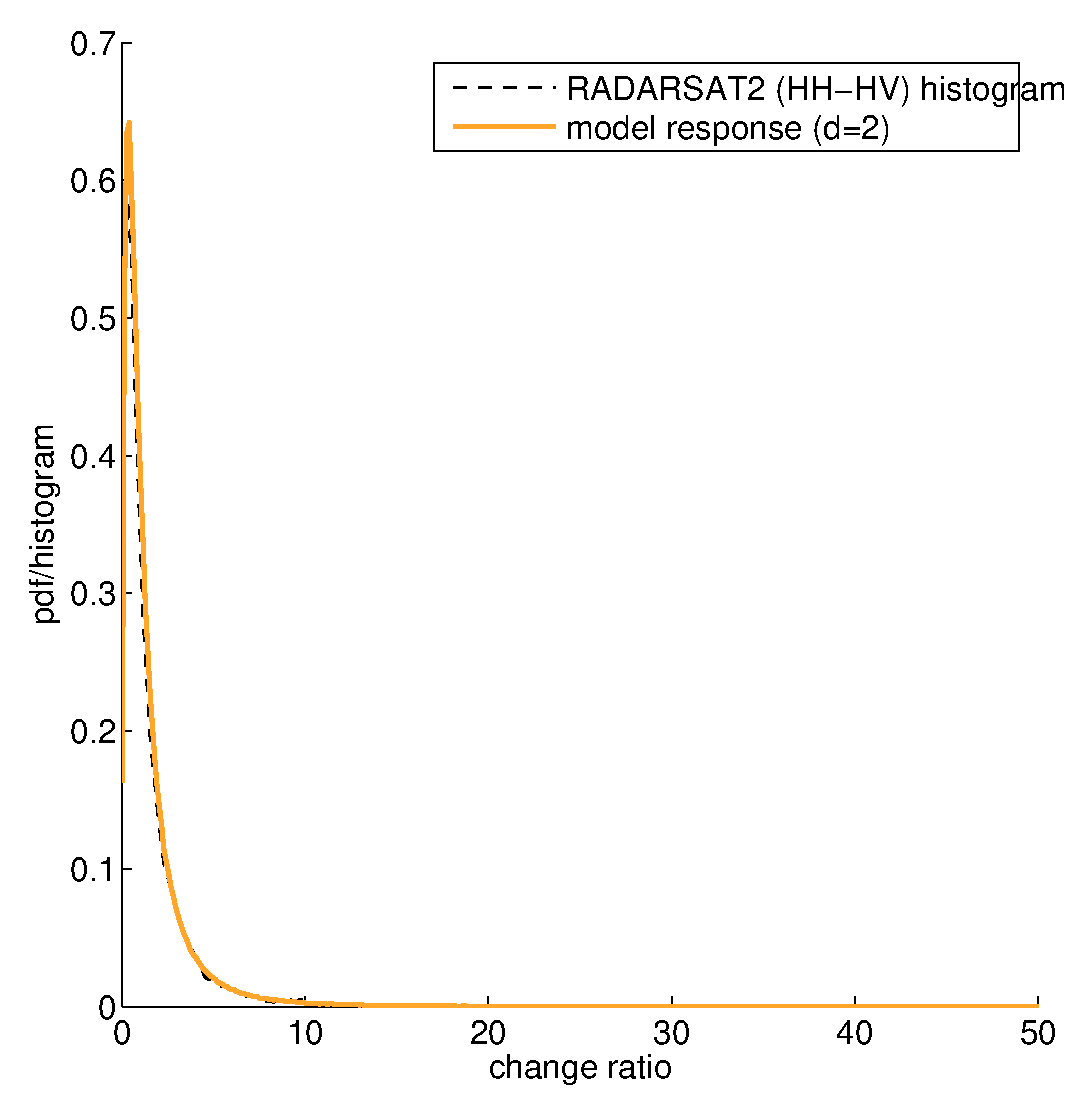
\includegraphics[width=1.5in,height=1.5in]{../images/verify_change_ratio_model_on_RADARSAT2_2d.eps}}
%          \begin{pspicture}[showgrid=false](\column,\row)% set showgrid=false for the final
%	    \rput[bl](0,0){\usebox\IBoxCRTwoR}
%	    \rput(5,1.5){\footnotesize{change-ratio}}
%	    \rput{90}(1.5,5){\footnotesize{pdf/histogram}}
%	    \psline[linecolor=plot](5,8)(6,8)
%	    \psline[linestyle=dashed](5,9)(6,9)%another line style: dotted
%	    \rput(8,8){\footnotesize{model}}
%	    \rput(8,9){\footnotesize{data}}
%          \end{pspicture}
%		 \epsfxsize=1.5in
%		 \epsfysize=1.5in
%		 \epsffile{../images/verify_change_ratio_model_on_RADARSAT2_2d.eps} 	
		 \label{RADARSAT2_2D_det_ratio}
	}
\end{tabular}
\caption{The specific $d=2$ models are validated on both RADARSAT2 and AIRSAR datasets}
\label{fig:verify_det_ratio_model_2D}
\end{figure}

\begin{figure}[h]
\centering
\begin{tabular}{c}
	\subfloat[AIRSAR (HH-HV-VV) determinant]{
          \plotWithLegend{../images/verify_determinant_model_on_AIRSAR_3d.eps}{determinant}
%		 \epsfxsize=1.5in
%		 \epsfysize=1.5in
%		 \epsffile{../images/verify_determinant_model_on_AIRSAR_3d.eps} 	
		 \label{AIRSAR_3D_determinant}
	} 
	\hfill	
	\subfloat[RADARSAT2 (HH-HV-VV) determinant]{
          \plotWithLegend{../images/verify_determinant_model_on_RADARSAT2_3d.eps}{determinant}
%		 \epsfxsize=1.5in
%		 \epsfysize=1.5in
%		 \epsffile{../images/verify_determinant_model_on_RADARSAT2_3d.eps} 	
		 \label{RADARSAT2_3D_determinant}
	} \\
	\subfloat[AIRSAR (HH-HV-VV) determinant ratio]{
          \plotWithLegend{../images/verify_det_ratio_model_on_AIRSAR_3d.eps}{determinant-ratio}
%		 \epsfxsize=1.5in
%		 \epsfysize=1.5in
%		 \epsffile{../images/verify_det_ratio_model_on_AIRSAR_3d.eps} 	
		 \label{AIRSAR_2D_det_ratio}
	} 
	\hfill	
	\subfloat[RADARSAT2 (HH-HV-VV) determinant ratio]{
          \plotWithLegend{../images/verify_det_ratio_model_on_RADARSAT2_3d.eps}{determinant-ratio}
%		 \epsfxsize=1.5in
%		 \epsfysize=1.5in
%		 \epsffile{../images/verify_det_ratio_model_on_RADARSAT2_3d.eps} 	
		 \label{RADARSAT2_2D_det_ratio}
	} \\
	\subfloat[AIRSAR (HH-HV-VV) change ratio]{
          \plotWithLegend{../images/verify_change_ratio_model_on_AIRSAR_3d.eps}{change-ratio}
%		 \epsfxsize=1.5in
%		 \epsfysize=1.5in
%		 \epsffile{../images/verify_change_ratio_model_on_AIRSAR_3d.eps} 	
		 \label{AIRSAR_2D_change_ratio}
	} 
	\hfill	
	\subfloat[RADARSAT2 (HH-HV-VV) change ratio]{
          \plotWithLegend{../images/verify_change_ratio_model_on_RADARSAT2_3d.eps}{change-ratio}
%          \begin{pspicture}[showgrid=false](\column,\row)% set showgrid=false for the final
%	    \rput[bl](0,0){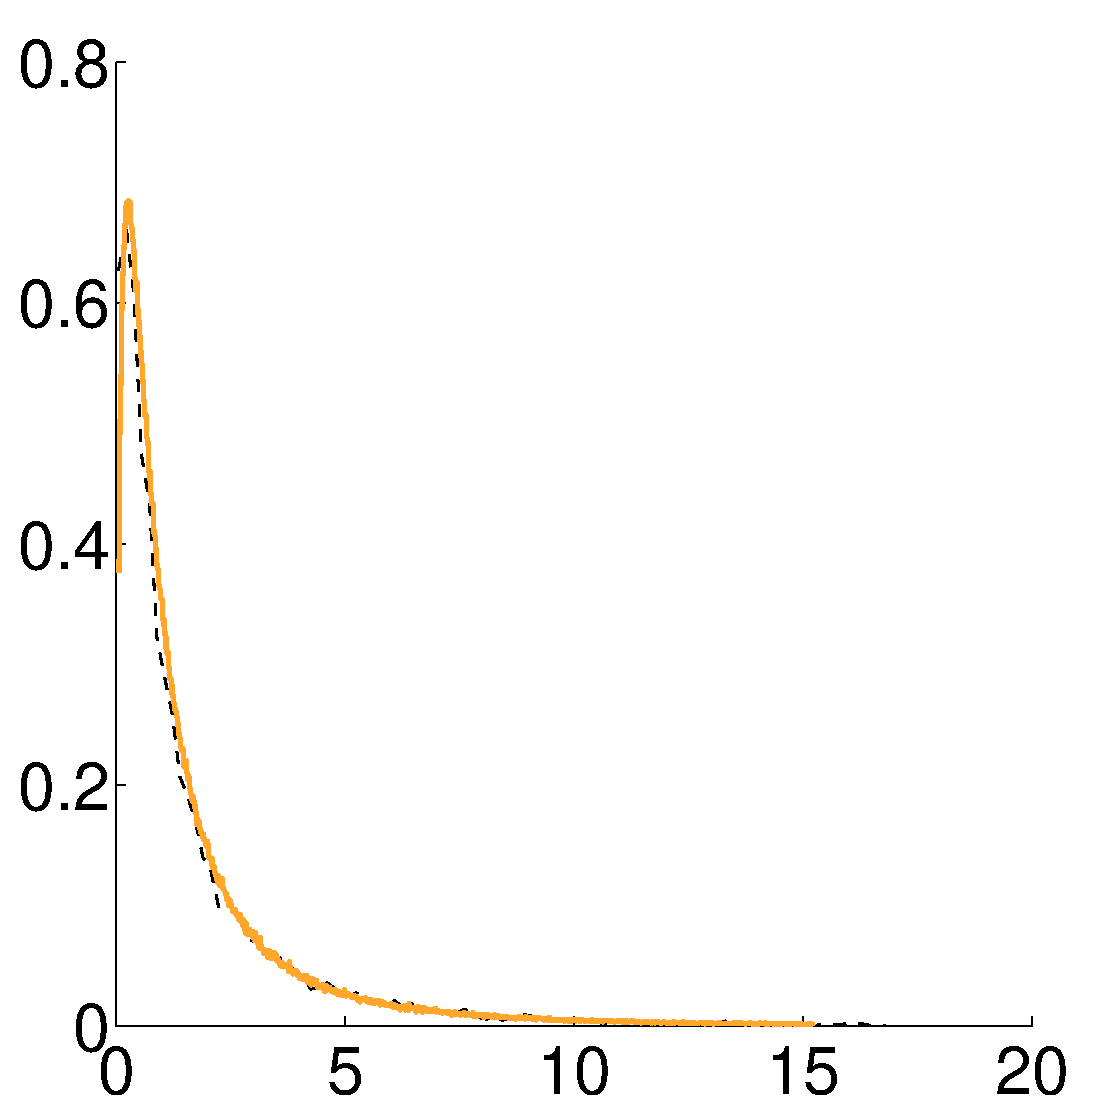
\includegraphics[width=1.5in,height=1.5in]{../images/verify_change_ratio_model_on_RADARSAT2_3d.eps}}% \usebox\IBoxCRThreeR
%	    \rput(5,1.5){\footnotesize{change-ratio}}
%	    \rput{90}(1.5,5){\footnotesize{pdf/histogram}}
%	    \psline[linecolor=plot](5,8)(6,8)
%	    \psline[linestyle=dashed](5,9)(6,9)%another line style: dotted
%	    \rput(8,8){\footnotesize{model}}
%	    \rput(8,9){\footnotesize{data}}
%          \end{pspicture}
%		 \epsfxsize=1.5in
%		 \epsfysize=1.5in
%		 \epsffile{../images/verify_change_ratio_model_on_RADARSAT2_3d.eps} 	
		 \label{RADARSAT2_2D_change_ratio}
	}
\end{tabular}
\caption{The specific $d=3$ models are validated on both practical RADARSAT2 and AIRSAR datasets}
\label{fig:verify_det_ratio_model_3D}
\end{figure}

%\subsection{Theoretical Implications of This Proposal}
\section{Discussion}
\label{sec:discussion}

%Let us begin by noting
To begin, a few theoretical properties of the proposed statistical models are discussed.
First, the use of covariance matrix log-determinant may be related to the standard eigen-decomposition method of the POLSAR covariance matrices.
In fact, the log-determinant can also be computed as the sum of log-eigenvalues.
Specifically $\ln{|M|} = \sum \ln{\lambda_M}$ where $\lambda_M$ denotes all the eigenvalues of $M$.
Thus, similar to other eigenvalue based approaches (e.g. entropy/anisotropy, ...),
  the models presented here are invariant to polarization basis transformations.

Second, the models are developed for the POLSAR covariance matrix.
However, since the POLSAR coherency matrix is related to the covariance matrix via a unitary transformation which preserves the determinant,
  the model is also applicable to the coherency matrix.

It should be noted that despite these advantages, the model descriptions are far from complete.
While it is desirable to reduce the multi-dimensional POLSAR data to a scalar value for many applications,
  such a reduction is unlikely to be lossless.  
Ideally %to better understand POLSAR data
the use of this technique could be complemented by some high-dimensional POLSAR target-decomposition techniques, such as the Freeman Durden decomposition \cite{Freeman_1998_TGRS_963} or the entropy/anisotropy decomposition \cite{Cloude_1997_TGRS_68} or similar.

Nevertheless the proposed models are promising.
Even though initially developed for partial and monostatic POLSAR data,
  it was shown to be applicable to traditional SAR data as well.
Since the model assumptions are quite minimal, they may potentially be applicable to bi-static and interferometric data, although that would require further study.

Intuitively, the concept of the determinant being representative of the POLSAR data can be thought of as being similar to the concept of using the magnitude to represent a complex number
(in a sense this is also why intensity is widely considered representative of the complex SAR data).
Similar to the determinant, the magnitude observable is also scalar and is not lossless, but it is undeniably useful.
To fully represent the complex number, another observable would needed besides the magnitude, for example a polar representation.
Magnitude is, of course, widely used as it can be shown to be invariant to a change in the reference frame.
Similarly, the determinant of the POLSAR covariance matrix is also scalar and invariant to a change of polarization basis.
Thus while it may not be \textit{fully} representative of the POLSAR data, it can be said to be \textit{highly} representative of it.
The important point is that it can provide a scalar comparison of the multi-dimensional data.
%**IVM removed this This is similar to the most commonly used magnitude to compare two or more complex numbers. %, most of the times the magnitude is to be used. 

Besides the above properties, the theoretical models may also provide an alternative derivation for the likelihood test statistics widely used in POLSAR.
Similar to the way that different measures of distance can be used to derive POLSAR classifiers \cite{Lee_1999_TGRS}, change detectors \cite{Conradsen_2003_TGRS_4}, edge detectors \cite{Schou_2003_TGRS_20} or other clustering and speckle filtering techniques \cite{Le_2010_ACRS} \cite{Le_2011_ACRS}, 
new detection, classification, clustering or speckle filtering algorithms can be derived using the models presented in this paper.
These applications however are not included in this paper, but rather left as a suggestion for future investigations.
%There are a few reasons for this decision.
%The first is that the advantages of the proposed models have been demonstrated through a few applications in this paper:
%  the first being a faster ENL evaluation for POLSAR data and
%  the second being the visual evaluation of POLSAR speckle filters.
%The second reason is that such an application would be quite big in scope, and as such would easily distract the reader from the main proposal of this paper.
%Last but not least, this paper focuses on the proposal of several scalar and representative statistical models for POLSAR, which results in associated statistical models and discrimination measures.
%It does not, technically speaking, focuses on proposing new discrimination measures.

%The advantages of this proposal are thus to be compared against other published models for POLSAR.
%Consequently, the methodology to evaluate the result of this proposal is a bit unusual.
%While quantitative evaluation is normally employed, in this theoretical model proposal only qualitative evaluation are shown.
%This is because compared to existing published observables for POLSAR, the advantage of the proposed observables are qualitative which does not requires numerical quantitative comparisons.
%Instead a straightforward binary evaluation would be sufficient.
%In comparison to other scalar models for POLSAR, the proposed models for determinant and its log-transformed version are representative are highly representative of the POLSAR data.
%This is because these models collapses into the representative SAR intensity when the multi-dimensional data is collapsed into the traditional one-dimensional SAR data.
%This is proven in section \ref{sec:sar_special_case_of_polsar}.
%No other existing models for POLSAR is known to have this property.
%
%Other advantage is that compared to other proposed scalar models for POLSAR, only these proposed statistical models lead to existing discrimination measures.
%This argument is supported by an extensive literature survey in section \ref{sec:lit_review}.
%There not only existing published scalar models for POLSAR are reviewed to show that none of them lead to discrimination measure,
%  existing discrimination measures for POLSAR are also extensively surveyed leaving virtually no chance of there exists an existing scalar statistical model for POLSAR which leads to existing discrimination measures.

%\section{Extending SAR data processing techniques towards POLSAR}
%
%Currently while the field of SAR is much more developed than the field of POLSAR,
%  the two fields however are quite separated.
%Hence many techniques applicable to SAR are not directly applicable to POLSAR.
%With the newly gained, the current proposal provide the bridge between these two separated fields,
%  inviting potential extension of various SAR processing techniques to POLSAR data.
%%For instance the earlier example illustrate that while intensity ratio was commonly used to carry out visually evaluation of SAR speckle filters,
%%  the newly proposed determinant ratio and its log-transformed version (i.e. contrast) are shown capable of visually evaluating POLSAR speckle filters.
%%We believe there are many more unexplored possibilities for such applications.
%  
%There are many beneficial implications for this proposal.
%One of the main benefits is that:
%  this proposal allows the extension of many of existing SAR data processing technique toward POLSAR.
%One example has already been presented in this paper, 
%  where existing SAR discrimination measures are extended towards POLSAR.
%Another example can be illustrated through an example which extends the SAR speckle filters evaluation technique towards POLSAR.  
%
%In evaluating SAR speckle filters, the intensity ratio is widely used.
%Specifically, in its original multiplicative domain, the ratio of the filtered output and the noisy input image represents the noise being removed.
%Assuming a perfect filtering condition, the ratio image should only contain random noise.
%Thus a commonly used visual evaluation is to simply plot the ratio image and determine if any image features have also been removed.
%
%Since the POLSAR determinant ratio has been shown to be equivalent to the SAR intensity ratio,
%  this technique can be equally applied to evaluate POLSAR speckle filters.
%In fact better results can be achieved.
%In \cite{Medeiros_2003_IJRS}, it has been shown that the multiplicative ratio is not  well suited to digital image presentation,
%  which is linear and additive in nature.
%Thus logarithmic transformation can be applied to convert the multiplicative determinant-ratio into the linear subtractive contrast.  
%NOTE: The above paragraph is long winding, should shortened it. I noted that that it is also used in the conclusion. Suggest remove it if possible)
%
%To demonstrate this feature, the technique is used to evaluate the performance of 3$\times$3 and 5$\times$5 boxcar POLSAR filters on the AIRSAR Flevoland partial polarimetric data (HH-HV).
%  A square 700$\times$700 pixel patch is first extracted from the AIRSAR dataset,
%  and the two POLSAR speckle filters are then applied to the patch.
%\footnote{While the boxcar filters may not stay in the frontier of POLSAR speckle filtering,
%  they are workable here since the focus of this experiment is not on finding the best POLSAR speckle filters available.
%  Rather its purpose is to show a quick example of how an existing technique in SAR data processing can be easily adapted for POLSAR data.} 
%The log-determinant images of the filtered outputs are displayed in Fig. \ref{fig:visual_eval_part_pol_boxcar_speckle_filters_3x3_vs_5x5}.
%At the same time, the residual is computed for both filters, and the images are also displayed in the same figure.
%
%%ifdef FINAL
%\begin{figure}[h]
%\centering
%\begin{tabular}{c}
%	\subfloat[Log-determinant Image of boxcar 3$\times$3 speckle filter]{
%		 \epsfxsize=1.5in
%		 \epsfysize=1.5in
%		 \epsffile{../images/visual_eval_part_pol_boxcar_3.filtered.eps} 	
%		 \label{multi_look_dispersion}
%	} 
%	\hfill	
%	\subfloat[Log-determinant Image of boxcar 5$\times$5 speckle filter]{
%		 \epsfxsize=1.5in
%		 \epsfysize=1.5in
%		 \epsffile{../images/visual_eval_part_pol_boxcar_5.filtered.eps} 	
%		 \label{multi_look_contrast}
%	} \\
%	\subfloat[Image of Log-determinant Residual for 3$\times$3 filter]{
%		 \epsfxsize=1.5in
%		 \epsfysize=1.5in
%		 \epsffile{../images/visual_eval_part_pol_boxcar_3.residual.eps} 	
%		 \label{multi_look_dispersion}
%	} 
%	\hfill	
%	\subfloat[Image of Log-determinant Residual for 5$\times$5 filter]{
%		 \epsfxsize=1.5in
%		 \epsfysize=1.5in
%		 \epsffile{../images/visual_eval_part_pol_boxcar_5.residual.eps} 	
%		 \label{multi_look_contrast}
%	} 
%\end{tabular}
%\caption{Visually Evaluating POLSAR Boxcar 3$\times$3 vs. 5$\times$5 Speckle Filters on AIRSA Flevoland part-pol data (HH-HV).}
%\label{fig:visual_eval_part_pol_boxcar_speckle_filters_3x3_vs_5x5}
%\end{figure}
%%endif
%%ifdef REVIEW
%\begin{figure}[h!]
%\centering
%\begin{tabular}{c}
%	\subfloat[Log-determinant Image of boxcar 3$\times$3 speckle filter]{
%		 \epsfxsize=3in
%		 \epsfysize=3in
%		 \epsffile{../images/visual_eval_part_pol_boxcar_3.filtered.eps} 	
%		 \label{multi_look_dispersion}
%	} 
%	\hfill	
%	\subfloat[Log-determinant Image of boxcar 5$\times$5 speckle filter]{
%		 \epsfxsize=3in
%		 \epsfysize=3in
%		 \epsffile{../images/visual_eval_part_pol_boxcar_5.filtered.eps} 	
%		 \label{multi_look_contrast}
%	} \\
%	\subfloat[Image of Log-determinant Residual for 3$\times$3 filter]{
%		 \epsfxsize=3in
%		 \epsfysize=3in
%		 \epsffile{../images/visual_eval_part_pol_boxcar_3.residual.eps} 	
%		 \label{multi_look_dispersion}
%	} 
%	\hfill	
%	\subfloat[Image of Log-determinant Residual for 5$\times$5 filter]{
%		 \epsfxsize=3in
%		 \epsfysize=3in
%		 \epsffile{../images/visual_eval_part_pol_boxcar_5.residual.eps} 	
%		 \label{multi_look_contrast}
%	} 
%\end{tabular}
%\caption{Visually Evaluating POLSAR Boxcar 3$\times$3 vs. 5$\times$5 Speckle Filters on AIRSAR Flevoland part-pol data (HH-HV).}
%\label{fig:visual_eval_part_pol_boxcar_speckle_filters_3x3_vs_5x5}
%\end{figure}
%%endif
%
%Fig. \ref{fig:visual_eval_part_pol_boxcar_speckle_filters_3x3_vs_5x5} shows that not only does the log-determinant image offer a nice visualization of the scene, 
%  the distortion impact of the filter can also be made visible by the residual image.
%In this visual evaluation, while it is quite hard to observe the worsen blurring-effects of the boxcar 5$\times$5 speckle filter compared to the 3$\times$3 filter
%in the additive log-determinant image of the filtered output, 
%  such an observation can be made relatively easier by inspecting the residual image.
%  
%There are many similar SAR data processing technique that may be adaptable to POLSAR.
%Examples in the same topic of evaluating speckle filters include
%  the use of the mean and variance of the ratio image, or ENL evaluation to quantitatively evaluate POLSAR speckle filters.
%Other topics that may also be connected include: speckle filtering, target detection, surface cover classification, edge detection ... and so on.

\section{Conclusion}
\label{sec:conclusion}

%What has been done?
This paper has proposed a generic statistical model  for the POLSAR covariance matrix determinant based on the complex Wishart POLSAR target vector distribution.%***IVM: Hai pls check this sentence!
This model has been validated for specific ($d=2$) and ($d=3$) using real-life partial and full polarimetric SAR data.
The paper also establishes a few POLSAR discrimination measures: the determinant-ratio and the change-ratio,  which essentially are the generic version of the SAR intensity-ratio.
At the same time, we have also shown a near-perfect match between the specific $d=1$ model and that for traditional SAR intensity,
  effectively bringing the existing SAR theories under the umbrella of this new model.

%What are the results? What are their advantages over others' results?
The main emphasis of this paper is the proposal to consider the POLSAR covariance matrix determinant as a scalar and representative observable for the multi-dimensional POLSAR data.
Compared to other published scalar observables, the determinant is highly representative of the multi-dimensional data.
Its representative power is justified for the following reasons.
Firstly, the covariance matrix determinant, when collapsed into one-dimensional case, transforms neatly into the representative SAR intensity.
Secondly, the statistical model for this observable is shown to be the generic multi-dimensional extension of the traditional model for the one dimensional SAR intensity.
Finally, this observable also leads to the establishment of the determinant-ratio discrimination measure for POLSAR data, which should increase the usability of this proposal.

%What are their benefit?
There are several beneficial implications of the proposed approach presented in this paper.
Currently while the field of SAR is much more developed than the field of POLSAR,  the two fields remain  quite separated.
Hence many techniques applicable to SAR can not be directly translated to POLSAR.
Since the scalar and representative model for POLSAR generalizes the traditional model for SAR intensity,
  its main benefit is that it enables the convenient adaptation of many existing SAR data processing techniques for POLSAR data.
One example has already been presented in this paper, 
  where existing SAR discrimination measures are extended towards POLSAR.
At the same time, it provides a consistent theory unifying the seemingly disparate discrimination measure proposals for SAR and POLSAR data.  

%What are their limitations? What problems this appears to solve, but actually is not?
Of course, the models proposed in this article also have their own limitations.
Firstly, they are based on the complex Wishart distribution
%Thus its applicability is also limited by that of its foundation,
%  that is the proposed theoretical model 
  which is only guaranteed to work for homogeneous areas.
Secondly, while it is desirable for a large number of applications to reduce the multi-dimensional POLSAR data to a scalar value, such a reduction is unlikely to be lossless in the general case.

In this paper, the theoretical model has only been validated for partial ($d=2$) and full ($d=3$) monostatic POLSAR data,
%and hence What can be done next?
  leaving the test of its validity for other datasets such as bistatic POLSAR data ($d=4$) or interferrometric POLSAR data ($d=6$) as possible future work.
Other possible future work includes
  an investigation on the applicability of this observables into POLSAR heterogeneous areas,
  as well as further studies to explore the use of these generic models in conjunction with other target decomposition techniques
    such as the Freeman-Durden decomposition \cite{Freeman_1998_TGRS_963} or the entropy/anisotropy decomposition \cite{Cloude_1997_TGRS_68}.

% references section
\bibliographystyle{IEEEtran}
\bibliography{IEEEabrv,article}

\end{document}
